\documentclass[../../main.tex]{subfiles}
\begin{document}
\section{Applicazioni alle derivate}
\subsection{Studio di funzioni}
Definiamo i punti di massimo e di minimo relativo.\\
Sia $f(x)$ definita in un intervallo $[a, b]$.
\begin{center}
    \begin{figure}[h!]
        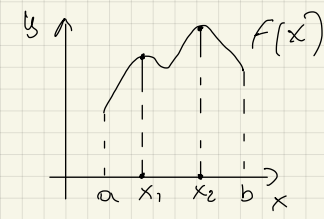
\includegraphics[scale=0.5]{studiofunzioni.png}
        \caption{f(x)}
        \label{fig:studiofunzioni}
    \end{figure}
\end{center}

\begin{itemize}
    \item $x_1\in[a, b]$ è un punto di \textbf{massimo relativo} per $f$ nell'intervallo $[a, b]$ se il valore $f(x_1)$ è più grande dei valori
          $f(x)$ per ogni $x$ nell'intervallo $[a, b]$ vicino ad $x_1$. Più precisamente se $\exists \delta > 0$
          tale che $f(x_1) \geq f(x)$ per ogni $x\in[a, b]$ tale che $|x-x_1|<\delta$.
    \item $x_2$ è un punto di \textbf{massimo assoluto} per $f$ se $f(x_2)\geq f(x)$ per ogni $x\in[a, b]$.
\end{itemize}
Analogamente per i punti di minimo con $\leq$ al posto di $\geq$.\\
\textbf{Osservazione:} Tutti i punti di massimo o minimo interni all'intervallo $[a, b]$ (cioè $\in(a, b)$) hanno retta tangente orizzontale in quel punto cioè del tipo:
\[
    y = q
\]
(Non vale per gli estremi per gli estremi dell'intervallo $x=a,b$, ma con $x_0\in(a, b)$).\\
Ricordando la retta tangente al grafico di una funzione in $x_0$
\[
    y = f(x_0) + f'(x_0)(x-x_0)
\]
questa retta è orizzontale $\iff f'(x_0) = 0$.\\

\subsection{Teorema di Fermat}
Sia $f$ una funzione definita in $[a, b]$ e sia $x_0$ un punto di massimo o di minimo relativo interno ad $[a, b]$.
Se $f$ è derivabile in $x_0$, allora risulta:
\[
    f'(x_0) = 0
\]
\textbf{Dimostrazione:} Supponiamo che $x_0$ sia un punto di massimo relativo, quindi $\exists \delta > 0$ tale che:
\[
    f(x_0) \geq f(x_0 + h) \ \ \ (\star) \ \ \forall h \ |h|<\delta \iff f(x_0)\geq f(x_0 + h) \ \ \forall x: |x-x_0|<\delta
\]
Valuto il rapporto incrementale:
\[
    \dfrac{f(x_0 + h) - f(x_0)}{h}
\]
il numeratore è sempre negativo perchè $x_0$ è \textbf{massimo} in $(\star)$.\\
E risulta:
\[
    \begin{cases}
        \leq 0 & \text{se } 0 < h < \delta  \\
        \geq 0 & \text{se } -\delta < h < 0
    \end{cases}
\]
e passando al limite per $h\to0^{\pm}$.\\
\[f'(x_0) = \lim_{h\to0^{\pm}}\dfrac{f(x_0 + h) - f(x_0)}{h} \leq 0\]
\[f'(x_0) = \lim_{h\to0^{\pm}}\dfrac{f(x_0 + h) - f(x_0)}{h} \geq 0\]
($f$ derivabile per ipotesi, quindi i due limiti devono coincidere).\\
Quindi $f'(x_0) = 0$. \ \ $\clubsuit$\\
\textbf{Osservazione:} Quindi conseguenza del teorema di Fermat è che l'annullamento della derivata prima di una funzione derivabile in un punto $x_0$ del dominio è condizione \textbf{necessaria} affichè
$x_0$ sia un punto di massimo o di minimo per la funzione.\\

\subsection{Teorema di Rolle}
Sia $f$ una funzione continua in $[a, b]$ e derivabile in $(a, b)$.\\
Se $f(a) = f(b)$, allora $\exists x_0\in(a, b)$ tale che $f'(x_0) = 0$.\\
\textbf{Dimostrazione:} Sia $f$ una funzione continua in $[a, b]$ quindi per il teorema di Weierstrass $f$ ammette massimo e minimo in $[a, b]$, cioè $\exists x_1, x_2\in[a, b]$ tali che:
\[
    f(x_1) \leq f(x) \leq f(x_2) \ \ \forall x\in[a, b] \ \ \ (\star)
\]
Se almeno uno fra $x_1$ e $x_2$ è un punto interno all'intervallo $[a, b]$ allora per il teorema di Fermat $f'(x_0) = 0$.\\

Rimane da esaminare il caso in cui entrambi i punti $x_1$ e $x_2$ non sono interni, cioè:
\[
    x_1 = a \ \ \text{e} \ \ x_2 = b
\]
Quindi da $(\star)$:
\[
    f(a) \leq f(x) \leq f(b) \ \ \forall x\in[a, b]
\]
Ma dato che per ipotesi $f(a) = f(b)$, $\implies$ significa che $f(x)$ è costante e la sua derivata è ovunque nulla.\\ \ \ $\clubsuit$\\

\subsection{Interpretazione geometrica}
$f(x)$ continua in $[a, b]$ e derivabile in $(a, b)$ con $f(a) = f(b)$, $\implies$ esiste un punto con tangente orizzontale.\\
% \begin{center}
%     \begin{tikzpicture}[line cap=round,line join=round,>=triangle 45,x=1.0cm,y=1.0cm]
%         \begin{axis}[
%                 x=1.0cm,y=1.0cm,
%                 axis lines=middle,
%                 ymajorgrids=true,
%                 xmajorgrids=true,
%                 xmin=-2.299520452224967,
%                 xmax=5.547670592618821,
%                 ymin=-0.9981723456395779,
%                 ymax=4.901036415184894,
%                 xtick={-2.0,-1.0,...,5.0},
%                 ytick={-0.0,1.0,...,4.0},]
%             \clip(-3.172822627595979,-1.560663093505579) rectangle (17.063915955074123,11.20715451600949);
%             \draw [shift={(4.,5.)},line width=2.pt]  plot[domain=0.:3.141592653589793,variable=\t]({1.*3.*cos(\t r)+0.*3.*sin(\t r)},{0.*3.*cos(\t r)+1.*3.*sin(\t r)});
%             \draw (0.9990071051572922,0.22245767936477323) node[anchor=north west] {$a$};
%             \draw (7.0044232930319605,0.18881389119740807) node[anchor=north west] {$b$};
%             \draw (-1.944824359487153,5.151272645883766) node[anchor=north west] {$f(a) = f(b)$};
%             \draw [line width=2.pt,dash pattern=on 4pt off 4pt] (0.,5.)-- (1.,5.);
%             \draw [line width=2.pt,dash pattern=on 4pt off 4pt] (1.,5.)-- (1.,0.);
%             \draw [line width=2.pt,dash pattern=on 4pt off 4pt] (7.,5.)-- (7.,0.);
%             \draw [line width=2.pt,domain=-3.172822627595979:17.063915955074123] plot(\x,{(--24.-0.*\x)/3.});
%             \begin{scriptsize}
%                 \draw [fill=ududff] (1.,5.) circle (2.5pt);
%                 \draw[color=ududff] (1.1167603637430699,5.31108063967875) node {$A$};
%                 \draw [fill=ududff] (7.,5.) circle (2.5pt);
%                 \draw[color=ududff] (7.122176551617739,5.31108063967875) node {$B$};
%                 \draw[color=black] (4.144701298805928,8.254912104323198) node {$c$};
%                 \draw [fill=xdxdff] (0.,5.) circle (2.5pt);
%                 \draw[color=xdxdff] (0.12426861280579987,5.31108063967875) node {$F$};
%                 \draw[color=black] (0.5448159648978634,4.890533287586686) node {$g$};
%                 \draw [fill=xdxdff] (1.,0.) circle (2.5pt);
%                 \draw[color=xdxdff] (1.1167603637430699,0.3149780968250273) node {$G$};
%                 \draw[color=black] (0.7803224820694191,2.6532213744569044) node {$h$};
%                 \draw [fill=xdxdff] (7.,0.) circle (2.5pt);
%                 \draw[color=xdxdff] (7.122176551617739,0.3149780968250273) node {$H$};
%                 \draw[color=black] (6.768916775860405,2.6532213744569044) node {$i$};
%                 \draw [fill=xdxdff] (4.,8.) circle (2.5pt);
%                 \draw[color=xdxdff] (4.111057510638563,8.305377786574246) node {$E$};
%                 \draw[color=black] (-2.9877817926754706,7.884830434482184) node {$f$};
%             \end{scriptsize}
%         \end{axis}
%     \end{tikzpicture}
% \end{center}
\textbf{Situazione più generale: }
\begin{center}

\end{center}
$\exists$ un punto $x_0\in(a,b)$, in cui la retta tangente è parallela alla corda che congiunge gli estremi del grafico
$(f(a) \text{ con } f(b))$.\\
\begin{itemize}
    \item $f'(x_0)$ coefficiente angolare della retta tangente in $x_0$.
    \item $\dfrac{f(b) - f(a)}{b-a}$ coefficiente angolare della corda.
\end{itemize}

\subsection{Teorema di Lagrange}
Sia $f(x)$ una funzione continua in $[a, b]$ e derivabile in $(a, b)$. Esiste un punto $x_0\in(a, b)$ per cui
\[
    f'(x_0) = \dfrac{f(b) - f(a)}{b-a}
\]
\textbf{Dimostrazione:} Si considera la funzione ausiliaria:
\[
    g(x) = f(x) - [f(a) + \dfrac{f(b) - f(a)}{b-a}(x-a)]
\]
\[
    \text{in }x = a \ \ \ g(a) = f(a) - [f(a) + \dfrac{f(b) - f(a)}{b-a}(a-a)] = 0
\]
\[
    \text{in }x = b \ \ \ g(b) = f(b) - [f(a) + \dfrac{f(b) - f(a)}{b-a}(b-a)] = 0
\]
\[
    \implies g(a) = g(b) = 0
\]
Posso quindi utilizzare il teorema di Rolle,
\[
    \exists x_0\in(a, b) \ \ \text{tale che} \ \ g'(x_0) = 0
\]
e
\[
    g'(x) = f'(x) - \dfrac{f(b) - f(a)}{b-a} \ \ \ \forall x\in(a, b)
\]
in $x_0 \implies$
\[
    f'(x_0) - \dfrac{f(b) - f(a)}{b-a} \ \ \ \clubsuit
\]

\subsection{Conseguenze del teorema di Lagrange}
\subsubsection{Criterio di monotonia}
Sia $f$ una funzione continua in $[a, b]$ e derivabile in $(a, b)$, allora:
\[
    \bullet f'(x) \geq 0 \ \ \forall x\in(a, b) \iff f \text{ è crescente in } [a, b]
\]
\[
    \bullet f'(x) \leq 0 \ \ \forall x\in(a, b) \iff f \text{ è decrescente in } [a, b]
\]
\textbf{Dimostrazione (per la prima):} Supponiamo che $\textcolor{purple}{f'(x) \geq 0}$ in $(a, b) \ \ \forall x\in(a, b)$, dobbiamo dimostrare che se
$a \leq x_1 < x_2 \leq b$ risulta $f(x_1) \leq f(x_2)$.\\
Applichiamo il Teorema di Lagrange nell'intervallo $[x_1, x_2]$:
\[
    \exists x_0\in(x_1, x_2) \ \ \text{tale che} \ \ f'(x_0) = \dfrac{f(x_2) - f(x_1)}{x_2 - x_1}
\]
Dato che $f'(x) \geq 0$ e $x_2 > x_1$ risulta $f(x_2) \geq f(x_1)$ e quindi $f$ è crescente. \\

Ora supponiamo $f$ crescente in $[a, b]$ e consideriamo $x$ e $x+h \in (a, b) \ \ (h>0)$ allora
$f(x+h) \geq f(x)$ per ipotesi e quindi:
\[
    \dfrac{f(x+h) - f(x)}{h} \geq 0
\]
e passando al limite:
\[
    f'(x) \geq 0 \ \ \ \forall x\in(a, b) \ \ \ \clubsuit
\]
\subsubsection{Caratterizzazione delle funzioni costanti in un intervallo}
Una funzione è costante in un intervallo $[a, b] \iff$ è derivabile in $[a, b]$ e la derivata è ovunque nulla.\\
\textbf{Dimostrazione:} Hp: $f(x)$ è costante in $[a, b] \implies f'(x) = 0$, lo abbiamo già visto con il rapporto incrementale
\[
    \dfrac{c-c}{h} = \dfrac{f(x+h) - f(x)}{h} = f(x) = c
\]
($\iff$) Se $f(x)$ è tale che $f'(x) = 0$ allora la funzione è costante.\\
Applico il Teorema di Lagrange nell'intervallo $[a, x] \implies \ \exists x_0\in(a,x)$ tale che:
\[
    0 = f'(x_0) = \dfrac{f(x)-f(a)}{x-a} \implies f(x) = f(a) \ \ \text{ cioè è costante} \ \ \clubsuit
\]


\subsection{Funzioni concave e convesse}
Si dice che una funzione è \textbf{convessa} in un intervallo $[a, b]$, se per ogni punto $x_0\in[a, b]$, il grafico della funzione
è \textbf{al di sopra} della retta tangente al grafico nel punto $(x_0. f(x_0))$\\
Si dice che una funzioneè \textbf{concava} in un intervallo $[a, b]$, se per ogni punto $x_0\in[a, b]$ il grafico della funzione è \textbf{al di sotto} della retta tangente
al grafico nel punto $(x_0, f(x_0))$.\\

$f$ convessa in $[a, b] \iff$
\[
    \begin{cases}
        f(x)\geq \textcolor{blue}{f(x_0) + f'(x_0)(x-x_0)} \\
        \forall x\in[a, b]
    \end{cases}
\]

$f$ concava in $[a, b] \iff$
\[
    \begin{cases}
        f(x)\leq \textcolor{blue}{f(x_0) + f'(x_0)(x-x_0)} \\
        \forall x\in[a, b]
    \end{cases}
\]
Un punto in cui $f(x)$ cambia la sua concavità è detto \textbf{punto di flesso}.

\subsubsection{Criterio di convessità}
Sia $f(x)$ una funzione derivabile in $[a, b]$ e che ammetta derivata seconda in $(a, b)$. Allora:\\
$f(x)$ è convessa in $[a, b] \iff$
\[
    f''(x) \geq 0 \ \ \forall x\in(a, b)
\]

\textbf{Osservazione:} $\iff f(x)$ è crescente in $[a, b]$ per il criterio di monotonia.

\subsection{Criterio per determinare se un punto è di massimo o minimo relativo per una funzione derivabile due volte} % (fold)
\begin{itemize}
    \item $f'(x_0) = 0$, $f''(x_0) > 0 \implies x_0$ è un punto di minimo relativo.
    \item $f'(x_0) = 0$, $f''(x_0) < 0 \implies x_0$ è un punto di massimo relativo.
\end{itemize}
Vediamo la prima, $f'(x_0) = 0$ e $f''(x_0) > 0$. SUpponendo che la derivata seconda sia continua in un intorno di $x_0$
(per il teorema della permanenza del segno) $f''(x)$ è positiva in un intorno di $x_0$, cioè in
$(x_0 - \delta, x_0 + \delta)$ con $\delta > 0$.\\
$\implies$ Quindi $f$ è convessa in tale intorno, per il criterio di convessità.
\[
    f(x)\geq f(x_0) \ \ \forall x\in(x_0 - \delta, x_0 + \delta)
\]
$\implies x_0$ è un punto di minimo relativo per $f$. \ \ $\clubsuit$

\subsection{Metodo di Newton per il calcolo delle radici di un'equazione}
E' un metodo per calcolare le radici di un'equazione $f(x) = 0$ con $f(x)$ funzione continua in un intervallo $[a, b]$ e tale che
$f(a) < 0$ e $f(b) > 0$.\\

\subsection{Metodo di Newton per il calcolo numerico approssimato degli zeri di una funzione}
In $[a, b]$, si sceglie un punto $x_1$ e si traccia la retta tangente al grafico della funzione per $x = x_1$.\\
Tale retta tangente incontrerà l'asse $x$ in un punto $x_2$, che sarà una approssimazione dello "zero" $x_0$ di $f(x)$.\\
L'equazione della retta tangente per $x = x_1$,
\[
    y = f(x_1) + f'(x_1)(x-x_1)
\]
Come si determina $x_2$? E' soluzione di
\[
    f(x_1) + f'(x_1)(x_2-x_1) = 0
\]
\[
    \implies x_2 = x_1 - \dfrac{f(x_1)}{f'(x_1)}
\]
Iteriamo. A partire da $x_2$ si considera nuovamente l'equazione della retta tangente al grafico di $f(x)$ per $x = x_2$:
\[
    y = f(x_2) + f'(x_2)(x-x_2)
\]
e si determina il punto $x_3$, dove questa retta tangente interseca l'asse $x$, come prima:
\[
    x_3 = x_2 - \dfrac{f(x_2)}{f'(x_2)}
\]
e
\[
    x_{n+1} = x_n - \dfrac{f(x_n)}{f'(x_n)}
\]
Si determina quindi una successione $x_n$ di approssimazioni del punto $x_0$.\\
In ipotesi abbastanza generali si dimostra che $x_n\to x_0$ per $n\to\infty$.\\
Si tratta di una successione \textbf{definita per ricorrenza}.\\
Applichiamo il metodo di Newton al calcolo approssimato delle cifre decimale di $\sqrt{2}$.
\subsection{Applicazione del metodo di Newton}
\subsubsection{Step 1}
Scegliamo, ad esempio, $x_1 = 2$ in $[0, 4]$, $f(x) = x^2 - 2$.
\[
    x_2 = x_1 - \dfrac{f(x_1)}{f'(x_1)} = 2 - \dfrac{2^2 - 2}{2\cdot2} = \dfrac{3}{2} = 1.5
\]
$\implies x_2 = 1.5$ è un'approssimazione per eccesso di $x_0 = \sqrt{2}$, cioè $x_2 > x_0$ perchè
$f(x)$ è \textbf{convessa} ($f'(x)=2$) e il suo grafico è \textbf{al di sopra}  di ogni sua retta tangente.\\
\subsubsection{Step 2}
Ripartiamo da $x_2 = 1.5$ e calcoliamo $x_3$:
\[
    x_3 = x_2 - \dfrac{f(x_2)}{f'(x_2)} = 1.5 - \dfrac{1.5^2 - 2}{2\cdot1.5} = \dfrac{17}{12} = 1.4166666666666667
\]
\subsubsection{Step n}
\[
    x_{n+1} = x_n - \dfrac{f(x_n)}{f'(x_n)}
\]
con $f(x) = x^2 - 2$ si trovano i valori:
\begin{center}
    \begin{tabular}{|c|c|}
        \hline
        $x_n$ & $approx$           \\
        \hline
        $x_1$ & 2                  \\
        $x_2$ & 1.5                \\
        $x_3$ & 1.4166666666666667 \\
        $x_4$ & 1.4142156862745097 \\
        $x_5$ & 1.4142135623746899 \\
        $x_6$ & 1.414213562373095  \\
        \hline
    \end{tabular}
\end{center}
La convergenza di $x_n$ a $x_0$, per $n\to\infty$ è molto rapida.\\
\[
    \sqrt{2} = 1.414213562373095\ldots
\]

\subsection{Teorema}
Sia $f(x)$ una funzione derivabile in $[a, b]$, con derivata continua e sia convessa in tale intervallo. Supponiamo
che $f(a) < 0$ e $f(b) > 0$ per ogni $x\in[a, b]$. Allora la successione definita per ricorrenza
\[
    x_1 = b \ \ \ \ \ x_{n+1} = x_n - \dfrac{f(x_n)}{f'(x_n)}
\]
converge decrescendo all'unica soluzione $x_0\in[a, b]$ dell'equazione $f(x) = 0$.\\
Nel caso studiato per il calcolo delle cifre decimali di $\sqrt{2}$, la successione
\[
    x_{n+1} = x_n - \dfrac{x_n^2 - 2}{2x_n} \text{ con } f(x) = x^2 - 2 \text{ e } f'(x) = 2x
\]
\[
    x_{n+1} = x_n - \dfrac{x_n^2 - 2}{2x_n} = x_n - \dfrac{x_n}{2} + \dfrac{1}{x_n}
\]
\[
    \implies \begin{cases}
        x_1 = 2 \\
        x_{n+1} = \dfrac{1}{2}x_n + \dfrac{1}{x_n}
    \end{cases}
    (\star)
\]
Verifichiamo che, se $x_n$ ammette limite finito, allora il limite è $\sqrt{2}$.\\
Infatti se $x_n \to x_0$, anche $x_{n+1} \to x_0$ e passando al limite in $(\star)$:
\[
    x_0 = \dfrac{1}{2}x_0 + \dfrac{1}{x_0} \implies 2x_0^2 = x_0^2 + 2 \implies x_0^2 = 2
\]
$\implies$ Quindi $x_0 = \pm \sqrt{2}$, ma essendo una successione a termini positivi (se $x_n > 0 \implies x_{n+1} = \frac{1}{2}x_n + \frac{1}{x_n} > 0$)\\
$\implies x_0 = \sqrt{2}$.\ \ $\clubsuit$

\subsection{Teorema di l'Hôpital}
Siano $f$ e $g$ funzioni derivabili in un intorno di $x_0$ (eventualmente anche non in $x_0$) tali che:
\[
    \lim_{x\to x_0} = 0 \ \ \ \ \ \ \lim_{x\to x_0}g(x) = 0
\]
Allora:
\[
    \frac{0}{0} \ \ \ \lim_{x\to x_0}\frac{f(x)}{g(x)} = \lim_{x\to x_0}\frac{f'(x)}{g'(x)}
\]
Se risulta $g(x) \neq 0$ e $g'(x) \neq 0$ in un intorno di $x_0, \ x\neq x_0$ e purchè esista il secondo limite.\\
\textbf{Osservazione:} Vale anche per forme indeterminate del tipo $\frac{\infty}{\infty}$. (Se $f(x), g(x) \to \infty$ per $x\to x_0$).
\subsection{Studio del grafico di una funzione}
\begin{enumerate}
    \item Determinare il Dominio della funzione
    \item Verificare la presenza di simmetria
          \begin{itemize}
              \item $f(x) = f(-x)$ funzione pari
              \item $f(-x) = -f(x)$ funzione dispari
              \item $f(x+T) = f(x)$ funzione periodica
          \end{itemize}
    \item Si determinano gli eventuali asintoti
\end{enumerate}

\subsubsection{Asintoti Verticali}
Una funzione ammette asintoto verticale, se calcolando il limite per $x\to x_0$ (oppure $x\to x_0^+$ e $x\to x_0^-$) si ottiene $\pm\infty$.
\[
    x = x_0 \text{ asintoto verticale } \iff \lim_{x\to x_0}f(x) = \pm\infty
\]
\subsubsection{Asintoti Orizzontali}
Una funzione ammette asintoto orizzontale, se calcolando il limite per $x\to\pm\infty$ si ottiene un valore finito.
\[
    y = l \text{ asintoto orizzontale } \iff \lim_{x\to\pm\infty}f(x) = l \in \R
\]

\subsubsection{Asintoti Obliqui}
Un asintoto obliquo per $x\to\pm\infty$ è una retta di equazione
\[
    y = mx + q
\]
\[
    \lim_{x\to\pm\infty}[f(x) - (mx + q)] = 0 \ \ \ (\star)
\]
(cioè per $x\to\pm\infty$ il grafico della funzione è vicino alla retta).\\
Dobbiamo determinare $m$ e $q$.\\
Se $(\star)\to0$, anche
\[
    \lim_{x\to\pm\infty}\dfrac{f(x) - (mx + q)}{x} = 0
\]
\[
    = \lim_{x\to\pm\infty}\dfrac{f(x)}{x} - m = 0
\]
\[
    \implies m = \lim_{x\to\pm\infty}\dfrac{f(x)}{x}
\]
\[
    \implies q = \lim_{x\to\pm\infty}[f(x) - mx]
\]
\textbf{Osservazione:} Se $f(x)$ ammette asintoto orizzontale allora non può ammettere asintoto obliquo, infatti:
\[
    \text{ HP } \ \ \lim_{x\to+\infty} = l \text{ ammette asintoto orizzontale}
\]
allora
\[
    m = \lim_{x\to\pm\infty}\dfrac{f(x)}{x} = = 0
\]
\[
    \implies q = \lim_{x\to\pm\infty}[f(x) - mx] = \lim_{x\to\pm\infty}f(x) = l
\]

\begin{enumerate}
    \setcounter{enumi}{3}
    \item Determinare gli intervalli dove la funzione è crescente o descrescente, i punti di massimo e di minimo relativo, \textbf{studiando il segno della derivata prima.}
    \item Si determinano gli intervalli dove la funzione è convessa o concava e gli eventuali punti di flesso, studiando il segno della derivata seconda.
\end{enumerate}






\end{document}